% Options for packages loaded elsewhere
\PassOptionsToPackage{unicode}{hyperref}
\PassOptionsToPackage{hyphens}{url}
%
\documentclass[
]{article}
\usepackage{amsmath,amssymb}
\usepackage{lmodern}
\usepackage{iftex}
\ifPDFTeX
  \usepackage[T1]{fontenc}
  \usepackage[utf8]{inputenc}
  \usepackage{textcomp} % provide euro and other symbols
\else % if luatex or xetex
  \usepackage{unicode-math}
  \defaultfontfeatures{Scale=MatchLowercase}
  \defaultfontfeatures[\rmfamily]{Ligatures=TeX,Scale=1}
\fi
% Use upquote if available, for straight quotes in verbatim environments
\IfFileExists{upquote.sty}{\usepackage{upquote}}{}
\IfFileExists{microtype.sty}{% use microtype if available
  \usepackage[]{microtype}
  \UseMicrotypeSet[protrusion]{basicmath} % disable protrusion for tt fonts
}{}
\makeatletter
\@ifundefined{KOMAClassName}{% if non-KOMA class
  \IfFileExists{parskip.sty}{%
    \usepackage{parskip}
  }{% else
    \setlength{\parindent}{0pt}
    \setlength{\parskip}{6pt plus 2pt minus 1pt}}
}{% if KOMA class
  \KOMAoptions{parskip=half}}
\makeatother
\usepackage{xcolor}
\IfFileExists{xurl.sty}{\usepackage{xurl}}{} % add URL line breaks if available
\IfFileExists{bookmark.sty}{\usepackage{bookmark}}{\usepackage{hyperref}}
\hypersetup{
  pdftitle={Step by Step Guide to Creating New Lessons},
  hidelinks,
  pdfcreator={LaTeX via pandoc}}
\urlstyle{same} % disable monospaced font for URLs
\usepackage[margin=1in]{geometry}
\usepackage{color}
\usepackage{fancyvrb}
\newcommand{\VerbBar}{|}
\newcommand{\VERB}{\Verb[commandchars=\\\{\}]}
\DefineVerbatimEnvironment{Highlighting}{Verbatim}{commandchars=\\\{\}}
% Add ',fontsize=\small' for more characters per line
\usepackage{framed}
\definecolor{shadecolor}{RGB}{248,248,248}
\newenvironment{Shaded}{\begin{snugshade}}{\end{snugshade}}
\newcommand{\AlertTok}[1]{\textcolor[rgb]{0.94,0.16,0.16}{#1}}
\newcommand{\AnnotationTok}[1]{\textcolor[rgb]{0.56,0.35,0.01}{\textbf{\textit{#1}}}}
\newcommand{\AttributeTok}[1]{\textcolor[rgb]{0.77,0.63,0.00}{#1}}
\newcommand{\BaseNTok}[1]{\textcolor[rgb]{0.00,0.00,0.81}{#1}}
\newcommand{\BuiltInTok}[1]{#1}
\newcommand{\CharTok}[1]{\textcolor[rgb]{0.31,0.60,0.02}{#1}}
\newcommand{\CommentTok}[1]{\textcolor[rgb]{0.56,0.35,0.01}{\textit{#1}}}
\newcommand{\CommentVarTok}[1]{\textcolor[rgb]{0.56,0.35,0.01}{\textbf{\textit{#1}}}}
\newcommand{\ConstantTok}[1]{\textcolor[rgb]{0.00,0.00,0.00}{#1}}
\newcommand{\ControlFlowTok}[1]{\textcolor[rgb]{0.13,0.29,0.53}{\textbf{#1}}}
\newcommand{\DataTypeTok}[1]{\textcolor[rgb]{0.13,0.29,0.53}{#1}}
\newcommand{\DecValTok}[1]{\textcolor[rgb]{0.00,0.00,0.81}{#1}}
\newcommand{\DocumentationTok}[1]{\textcolor[rgb]{0.56,0.35,0.01}{\textbf{\textit{#1}}}}
\newcommand{\ErrorTok}[1]{\textcolor[rgb]{0.64,0.00,0.00}{\textbf{#1}}}
\newcommand{\ExtensionTok}[1]{#1}
\newcommand{\FloatTok}[1]{\textcolor[rgb]{0.00,0.00,0.81}{#1}}
\newcommand{\FunctionTok}[1]{\textcolor[rgb]{0.00,0.00,0.00}{#1}}
\newcommand{\ImportTok}[1]{#1}
\newcommand{\InformationTok}[1]{\textcolor[rgb]{0.56,0.35,0.01}{\textbf{\textit{#1}}}}
\newcommand{\KeywordTok}[1]{\textcolor[rgb]{0.13,0.29,0.53}{\textbf{#1}}}
\newcommand{\NormalTok}[1]{#1}
\newcommand{\OperatorTok}[1]{\textcolor[rgb]{0.81,0.36,0.00}{\textbf{#1}}}
\newcommand{\OtherTok}[1]{\textcolor[rgb]{0.56,0.35,0.01}{#1}}
\newcommand{\PreprocessorTok}[1]{\textcolor[rgb]{0.56,0.35,0.01}{\textit{#1}}}
\newcommand{\RegionMarkerTok}[1]{#1}
\newcommand{\SpecialCharTok}[1]{\textcolor[rgb]{0.00,0.00,0.00}{#1}}
\newcommand{\SpecialStringTok}[1]{\textcolor[rgb]{0.31,0.60,0.02}{#1}}
\newcommand{\StringTok}[1]{\textcolor[rgb]{0.31,0.60,0.02}{#1}}
\newcommand{\VariableTok}[1]{\textcolor[rgb]{0.00,0.00,0.00}{#1}}
\newcommand{\VerbatimStringTok}[1]{\textcolor[rgb]{0.31,0.60,0.02}{#1}}
\newcommand{\WarningTok}[1]{\textcolor[rgb]{0.56,0.35,0.01}{\textbf{\textit{#1}}}}
\usepackage{graphicx}
\makeatletter
\def\maxwidth{\ifdim\Gin@nat@width>\linewidth\linewidth\else\Gin@nat@width\fi}
\def\maxheight{\ifdim\Gin@nat@height>\textheight\textheight\else\Gin@nat@height\fi}
\makeatother
% Scale images if necessary, so that they will not overflow the page
% margins by default, and it is still possible to overwrite the defaults
% using explicit options in \includegraphics[width, height, ...]{}
\setkeys{Gin}{width=\maxwidth,height=\maxheight,keepaspectratio}
% Set default figure placement to htbp
\makeatletter
\def\fps@figure{htbp}
\makeatother
\setlength{\emergencystretch}{3em} % prevent overfull lines
\providecommand{\tightlist}{%
  \setlength{\itemsep}{0pt}\setlength{\parskip}{0pt}}
\setcounter{secnumdepth}{-\maxdimen} % remove section numbering
\ifLuaTeX
  \usepackage{selnolig}  % disable illegal ligatures
\fi

\title{Step by Step Guide to Creating New Lessons}
\author{}
\date{\vspace{-2.5em}2023-02-11}

\begin{document}
\maketitle

\emph{Please note: you'll need to have Git installed on your computer
and the distill package installed first}

\hypertarget{step-1-create-your-lesson-plan}{%
\section{Step 1: Create your lesson
plan}\label{step-1-create-your-lesson-plan}}

The very first step is to put together your RGirls lesson plan! To do
this, we recommend using the RGirls lesson plan template. To do this,
please follow along with the steps below.

\begin{itemize}
\tightlist
\item
  Install and load in the RGirls package
\end{itemize}

\begin{Shaded}
\begin{Highlighting}[]
\NormalTok{devtools}\SpecialCharTok{::}\FunctionTok{install\_github}\NormalTok{(}\StringTok{"R{-}Girls/RGirls"}\NormalTok{)}
\FunctionTok{library}\NormalTok{(RGirls)}
\end{Highlighting}
\end{Shaded}

\begin{itemize}
\tightlist
\item
  Go to the \href{https://github.com/R-Girls/RGirls}{RGirls GitHub
  Repository} and follow along with the steps under ``Lesson plan
  template''
\end{itemize}

\emph{If you just installed the RGirls package and can't find the
rgirlspdf, try restarting R or even closing and reopening RStudio}

\begin{itemize}
\item
  Modify the file as needed to incorporate your new lesson plan
\item
  Knit the file to make sure everything looks good
\item
  At this point, I recommend saving your lesson plan somewhere safe on
  your computer and we will come back to it later
\end{itemize}

\hypertarget{step-2-clone-github-repository}{%
\section{Step 2: Clone GitHub
repository}\label{step-2-clone-github-repository}}

\textbf{You will only need to do this step one time. Once you follow
these steps and set up your R Project, you can add and modify as many
lessons as you'd like.}

In order to add your lesson plan to the website, the next thing you need
to do is clone the \textbf{RGirls Website} Repository (please note this
is a different repository than the one we used to create our lesson
plan) to your local computer. We will do this by setting up a version
control R project through Git. This will allow you to work in RStudio on
your computer and push updates to GitHub, which will in turn update the
website.

\begin{itemize}
\item
  Navigate to the \href{https://github.com/R-Girls/website}{RGirls
  Website GitHub Repository}
\item
  Click the green code button and copy the URL
\end{itemize}

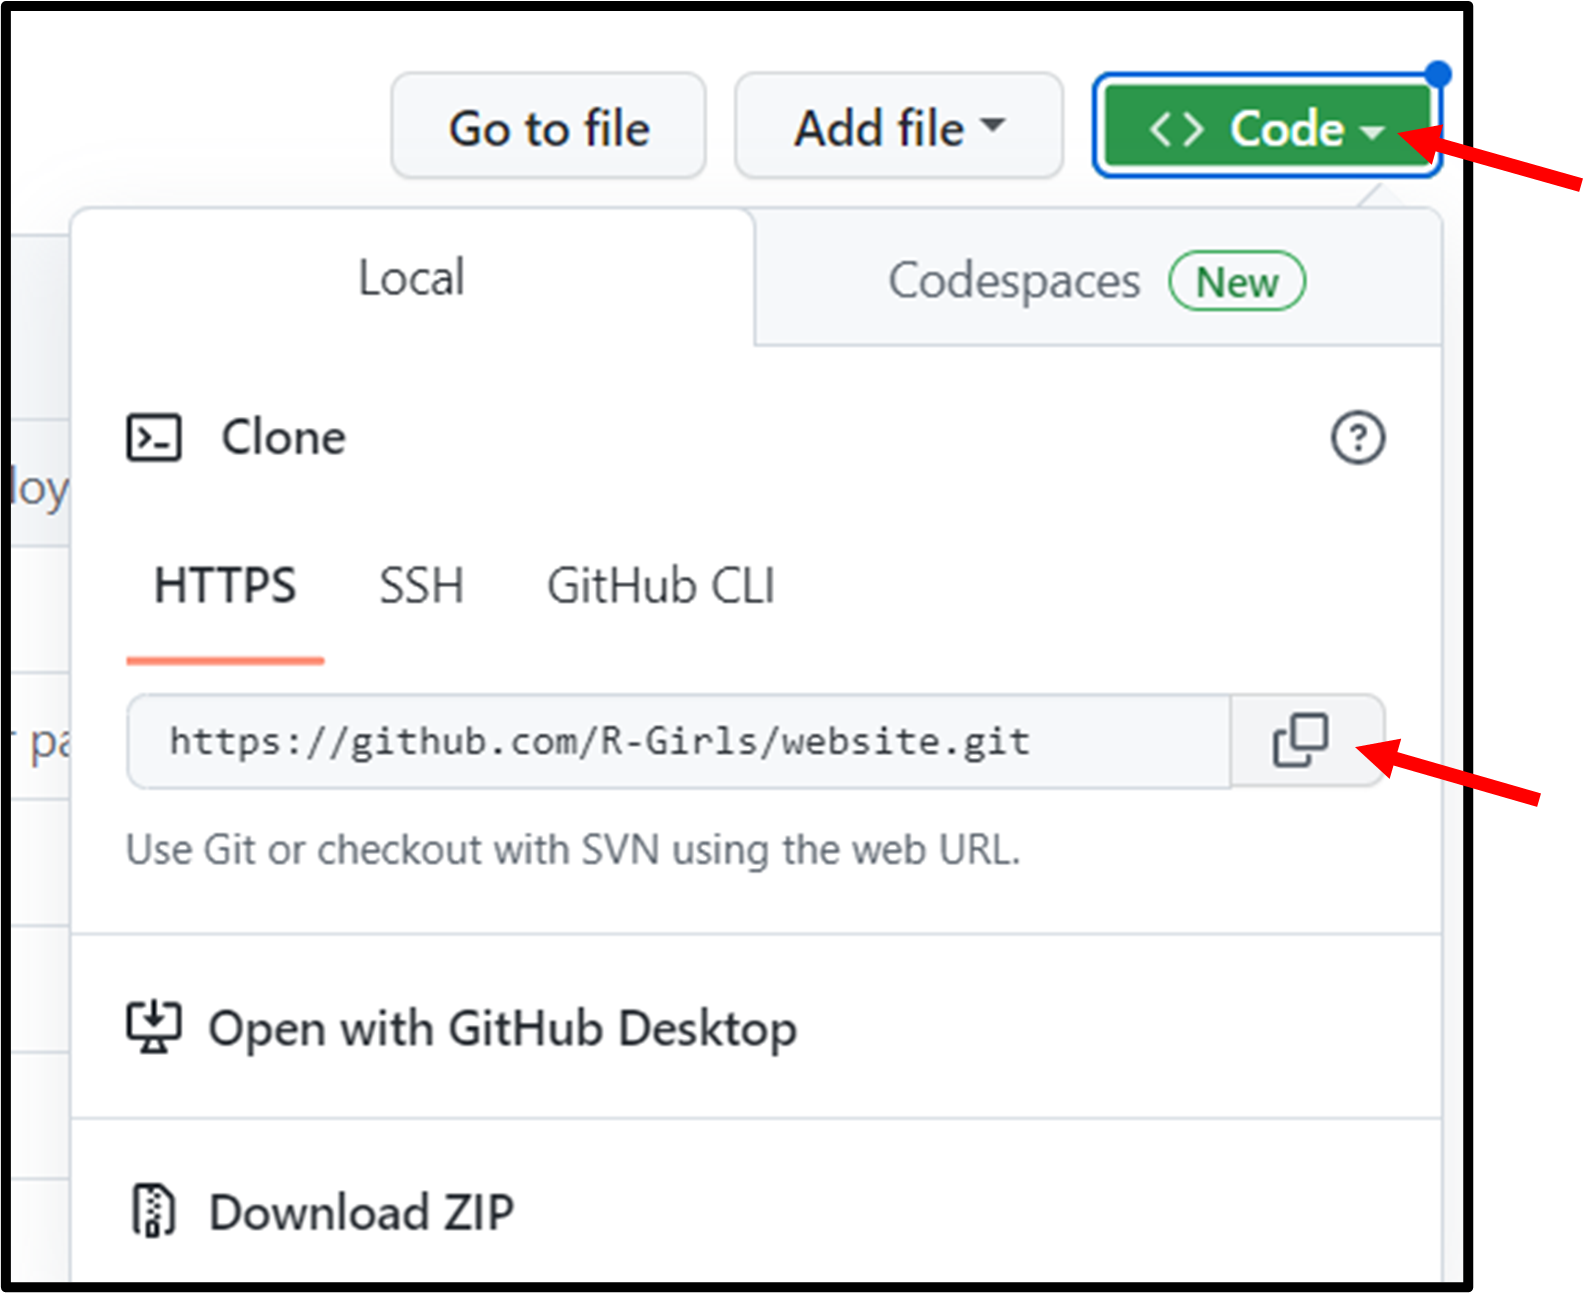
\includegraphics[width=0.4\textwidth,height=\textheight]{images/guide-img1.png}

\begin{itemize}
\tightlist
\item
  Open RStudio and in the top right corner, click on the ``Project''
  button and select New Project
\end{itemize}

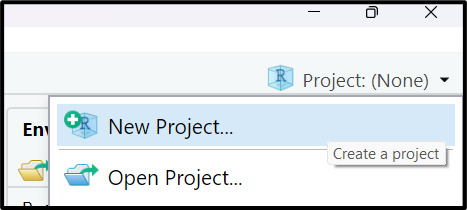
\includegraphics[width=0.4\textwidth,height=\textheight]{images/guide-img2.png}

\begin{itemize}
\tightlist
\item
  Then click Version Control -\textgreater{} Git -\textgreater{} and
  paste the URL that you copied from GitHub. a. Make sure to click on
  browse to save your project to a safe location on your computer.
\end{itemize}

\hypertarget{step-3-understanding-the-file-structure}{%
\section{Step 3: Understanding the file
structure}\label{step-3-understanding-the-file-structure}}

Now you should have your own clone of the RGirls Website repository. In
other words, you have a new R Project that contains all of the files to
create the RGirls website. Because this project was created through Git,
you can make updates and changes in order to update the website. Before
moving on to adding your new lesson plan to the website, let's take a
few minutes to understand the file structure of this project. Your files
tab should look similar to this (although files and folders may be
updated)

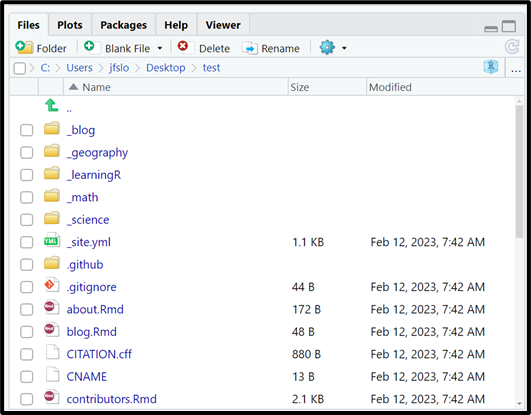
\includegraphics[width=0.4\textwidth,height=\textheight]{images/guide-img-file-structure.png}

The folders at the top with the underscore are the different ``posts''
that have already been created. A post is a distill term, which is
essentially a unique category of blogs or lessons that you want to
share. For example, on the RGirls website we have a ``Blog'' tab with
RGirls blogs. You can find these blogs in the \texttt{\_blog} folder.
There are also folders for the different categories of lessons (e.g.,
math, science, geography, etc.).

Just as a heads up: when you create a new post in distill, you have to
specify which ``collection'' (aka which folder) you want to add your
lesson to. For example, if you are creating a new Math lesson, you'll
want to add it to the \texttt{\_math} folder. Once you add your lesson,
it will be updated on the website and your new post will be at the top
of the page.

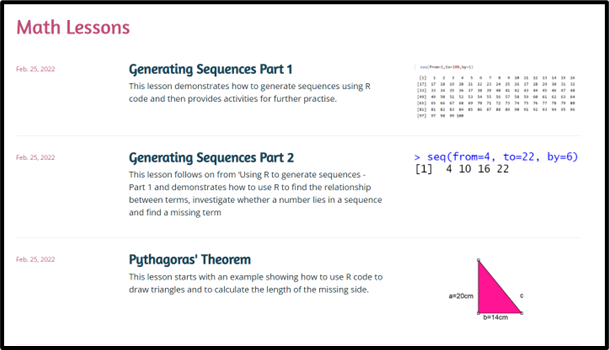
\includegraphics[width=0.4\textwidth,height=\textheight]{images/guide-img-math-lesson.png}

There are a lot of other folders and a few other folders in our project,
but for the purposes of creating a new lesson, we will not worry about
everything else. You are welcome to explore the different folders and
files, but please do not make any changes to the other files as we do
not want to accidentally break anything on the website.

\hypertarget{create-new-lesson-post}{%
\section{Create New Lesson Post}\label{create-new-lesson-post}}

Okay, now we are ready to create a new post so we can add our lesson
plan to the RGirls website.

\textbf{I recommend following along with my
\href{https://www.youtube.com/watch?v=b7TLIX6z1JQ}{YouTube Tutorial}
starting at 10:03}

\begin{itemize}
\tightlist
\item
  First, make sure to have the distill package installed and loaded in
\end{itemize}

\begin{Shaded}
\begin{Highlighting}[]
\CommentTok{\# install.packages("distill")}
\FunctionTok{library}\NormalTok{(distill)}
\end{Highlighting}
\end{Shaded}

\hypertarget{create_post}{%
\subsection{\texorpdfstring{\texttt{create\_post()}}{create\_post()}}\label{create_post}}

\begin{itemize}
\item
  In the console, use the \texttt{create\_post()} function (this is a
  Distill function) to create your new lesson

  \begin{itemize}
  \item
    The first argument you need to specify is the title. I recommend
    adding ``\_post'' to your title as a way to remember this is the
    lesson post which is different from your .Rmd file that you created
    from the RGirls template.
  \item
    The second argument you need to specify is the collection. This will
    save your lesson to the correction location. Currently, the possible
    collections are (even though the folders in our directory are
    written with an underscore, do not use an underscore here):

    \begin{itemize}
    \tightlist
    \item
      ``math''
    \item
      ``science''
    \item
      ``geography''
    \end{itemize}
  \item
    Press enter to run this code in your console
  \end{itemize}
\end{itemize}

\textbf{For purposes of this guide, I'll pretend to create a math lesson
called ``test''}

\begin{Shaded}
\begin{Highlighting}[]
\FunctionTok{create\_post}\NormalTok{(}\AttributeTok{title =} \StringTok{"test\_post"}\NormalTok{, }\AttributeTok{collection =} \StringTok{"math"}\NormalTok{)}
\end{Highlighting}
\end{Shaded}

\textbf{If you wish to add a new category (aka collection), you can
follow along with my
\href{https://www.youtube.com/watch?v=b7TLIX6z1JQ}{YouTube Tutorial}
starting at 7:10.}

\begin{itemize}
\item
  You'll see an .Rmd file (\texttt{testpost.Rmd}) will automatically pop
  up. This is the .Rmd file of your new lesson for the website! Don't
  worry about editing the content just yet, we'll come back to this .Rmd
  file in a minute.
\item
  You can also navigate to the folder of the category of your lesson
  (e.g., \_math if you are creating a math lesson) and there will be a
  new folder with today's date and the title of your lesson. Click on
  the folder and you will see where the .Rmd file is saved.
\end{itemize}

\hypertarget{upload-your-.rmd-lesson-plan}{%
\subsection{Upload your .Rmd lesson
plan}\label{upload-your-.rmd-lesson-plan}}

Now that we have our folder created for our new lesson, let's add our
.Rmd lesson plan that we created in Step 1. I find it easiest to do this
outside of RStudio.

\begin{itemize}
\item
  Outside of RStudio, navigate to where you have saved this R Project
\item
  Open the folder that you just created for your new lesson (e.g., my
  test folder would be called ``YYYY-MM-DD-testpost'')
\item
  Make a copy of your beautiful lesson plan and save it in your new post
  folder. I recommend saving it with a similar name as the other .Rmd
  file in this folder excluding ``post''. So for me, I had
  \texttt{testpost.Rmd} and now I'll save my actual lesson as
  \texttt{test.Rmd}. I know this is a little confusing, but to try to
  clarify:

  \begin{itemize}
  \tightlist
  \item
    The \texttt{test.Rmd} is your ``clean'' lesson that follows the
    lesson template. This will also be the .Rmd file that people can
    download directly from the website.
  \item
    The \texttt{testpost.Rmd} is similar because it will eventually have
    the code to the lesson too, but it will also have extra code that is
    necessary for the lesson plan to integrate with the website and
    display properly online.
  \end{itemize}
\item
  This is a good time to upload any other necessary files for your
  lesson post. For example, some of the previous lessons have word docs
  and pdfs available for download directly from the website. As an
  example, see the screenshot below of the Boxplot lesson plan - note
  that this lesson plan has an .Rmd, a word doc, and a pdf that you can
  download straight from the website. In order to download these files,
  they need to be saved in your lesson folder. So, if you wish to add
  any files like this, make sure to upload them to this folder now.
\end{itemize}

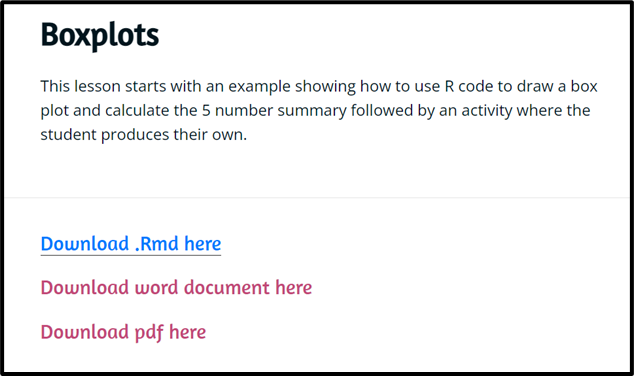
\includegraphics[width=0.4\textwidth,height=\textheight]{images/guide-img3.png}

\hypertarget{update-your-lesson-post}{%
\subsection{Update your lesson post}\label{update-your-lesson-post}}

Now that you have your beautiful lesson plan created and saved in the
correct location, we can update the \texttt{testpost.Rmd} file. I
recommend opening another existing post to see how it's formatted. For
example, go to \texttt{\_math} -\textgreater{}
\texttt{2022-03-11-boxplotpost} -\textgreater{} and open
\texttt{boxplotpost.Rmd}. Please don't modify this code, but it will be
useful to reference as you go through the next several steps.

\begin{itemize}
\item
  To start, open up the \texttt{testpost.Rmd} file
\item
  Edit the code in the YAML (which is the code in between the --- at the
  top of the .Rmd file)

  \begin{itemize}
  \tightlist
  \item
    Do not delete this code
  \item
    Rather, modify it with the correct content. For example, add the
    title of your lesson plan and a brief description that you'll want
    to show up on the website.
  \item
    You can always comment out a line of code in the YAML if you do not
    want to include it. For example \texttt{\#author:\ {[}{]}} if you
    don't want to include an author.
  \end{itemize}
\item
  Directly under the YAML add the following lines of code which will
  create the links on the website for people to download a copy of your
  lesson plan (this code should \textbf{not} be placed inside an R
  chunk):

  \begin{itemize}
  \item
    Modify this code to make sure the
    \texttt{here("\_math",\ "YYYY-MM-DD-testpost",\ "test.Rmd"),\ text\ =\ "Download\ .Rmd\ here")}
    function has all of the correct information:

    \begin{itemize}
    \tightlist
    \item
      The first argument should be the correct collection (e.g., \_math,
      \_science, \_geography)
    \item
      The second argument should be the name of the folder that was
      created when you ran \texttt{create\_post()} (e.g.,
      ``2022-03-11-boxplotpost'')
    \item
      The third argument should be the actual file you want to download.
      Make sure to have the files saved in this folder
    \end{itemize}
  \end{itemize}
\end{itemize}

\begin{Shaded}
\begin{Highlighting}[]
\SpecialCharTok{\textless{}}\NormalTok{div class}\OtherTok{=}\StringTok{"contributor\_org"}\SpecialCharTok{\textgreater{}}
\StringTok{\textasciigrave{}}\AttributeTok{r xfun::embed\_file(here::here("\_math", "YYYY{-}MM{-}DD{-}testpost", "test.Rmd"), text = "Download .Rmd here")}\StringTok{\textasciigrave{}}

\StringTok{\textasciigrave{}}\AttributeTok{r xfun::embed\_file(here::here("\_math", "YYYY{-}MM{-}DD{-}testpost", "test.docx"), text = "Download word document here")}\StringTok{\textasciigrave{}}

\StringTok{\textasciigrave{}}\AttributeTok{r xfun::embed\_file(here::here("\_math", "YYYY{-}MM{-}DD{-}testpost", "test.pdf"), text = "Download pdf here")}\StringTok{\textasciigrave{}}
\SpecialCharTok{\textless{}}\ErrorTok{/}\NormalTok{div}\SpecialCharTok{\textgreater{}}
\end{Highlighting}
\end{Shaded}

\begin{itemize}
\tightlist
\item
  Let's say you only have the .Rmd file that you want to make available
  to download. No problem! Only include the code:
\end{itemize}

\begin{Shaded}
\begin{Highlighting}[]
\SpecialCharTok{\textless{}}\NormalTok{div class}\OtherTok{=}\StringTok{"contributor\_org"}\SpecialCharTok{\textgreater{}}
\StringTok{\textasciigrave{}}\AttributeTok{r xfun::embed\_file(here::here("\_math", "YYYY{-}MM{-}DD{-}testpost", "test.Rmd"), text = "Download .Rmd here")}\StringTok{\textasciigrave{}}
\SpecialCharTok{\textless{}}\ErrorTok{/}\NormalTok{div}\SpecialCharTok{\textgreater{}}
\end{Highlighting}
\end{Shaded}

\begin{itemize}
\item
  The rest of the \texttt{testpost.Rmd} file will contain your lesson
  plan. So, go to \texttt{test.Rmd} and copy all the code excluding the
  YAML and paste it under the \texttt{\textless{}/div\textgreater{}} tag
\item
  Finally, after the \#\#THE END of your lesson add the following code
  for information about the license and citation (again, do \textbf{not}
  put this in an R chunk)
\end{itemize}

\begin{Shaded}
\begin{Highlighting}[]
\SpecialCharTok{\textless{}}\NormalTok{div class}\OtherTok{=}\StringTok{"license"}\SpecialCharTok{\textgreater{}}
\ErrorTok{**}\NormalTok{License and Citation}\SpecialCharTok{:}\ErrorTok{**}\NormalTok{ You can use, modify, and adapt any of the lessons, but please include the following attribution}\SpecialCharTok{:} \ErrorTok{*}\NormalTok{RGirls }\FunctionTok{Community.}\NormalTok{ (}\DecValTok{2022}\NormalTok{, April }\DecValTok{10}\NormalTok{). RGirls Lessons. Zenodo. [https}\SpecialCharTok{:}\ErrorTok{//}\NormalTok{doi.org}\SpecialCharTok{/}\FloatTok{10.5281}\SpecialCharTok{/}\NormalTok{zenodo}\FloatTok{.6436861}\NormalTok{](https}\SpecialCharTok{:}\ErrorTok{//}\NormalTok{doi.org}\SpecialCharTok{/}\FloatTok{10.5281}\SpecialCharTok{/}\NormalTok{zenodo}\FloatTok{.6436861}\NormalTok{)}\SpecialCharTok{*} 
\ErrorTok{\textless{}/}\NormalTok{div}\SpecialCharTok{\textgreater{}}
\end{Highlighting}
\end{Shaded}

\hypertarget{see-if-everything-worked}{%
\section{See if everything worked}\label{see-if-everything-worked}}

\begin{itemize}
\item
  Once you're happy with the content of your lesson plan, make sure to
  knit the file (the \texttt{testpost.Rmd} file). As soon as you knit
  your file, it will create a .html file of your lesson, which is
  necessary in order to add it to the website.
\item
  It's a good sing if you were able to knit your file with no errors,
  but now let's try to build our website.
\item
  In the top right hand corner, go to the Build tab and click Build
  Website
\item
  If the website pops up in the Viewer pane of RStudio click on the
  ``show in new window'' button directly next to the broom
\item
  Go to the Math Lessons tab (or whichever category your new lesson
  falls under) and make sure your lesson is there. It should be at the
  top because it's ordered by date.
\item
  Click on your lesson plan and make sure everything looks good. Things
  to check for:

  \begin{itemize}
  \tightlist
  \item
    Make sure the description is there
  \item
    Make sure you can successfully download the files (if you included
    any to download)
  \item
    Make sure the lesson plan is all there
  \item
    Make sure the license and citation text is there
  \end{itemize}
\end{itemize}

\emph{If you don't see your lesson plan, go back to your
\texttt{testpost.Rmd} and knit the file. And then try to build your site
again and see if it works}

\hypertarget{push-changes-to-github}{%
\section{Push Changes to GitHub}\label{push-changes-to-github}}

\textbf{You can follow along with my
\href{https://www.youtube.com/watch?v=b7TLIX6z1JQ}{YouTube Tutorial}
starting at 20:05.}

\textbf{If this is your first time connecting to GitHub from RStudio,
you can following along with
\href{https://www.youtube.com/watch?v=NLU05CopNzU}{this YouTube
Tutorial} starting at 15:40.}

Now that we confirmed that the new lesson is working on our local
computer, we need to push all the changes to GitHub so the actual
website will be updated.

To do this we need to do three things: Stage, Commit, and Push.

\begin{enumerate}
\def\labelenumi{\arabic{enumi}.}
\item
  Stage: at the top bar, go to Tools -\textgreater{} Shell and type
  ``git add -A'' in the command line and push enter. This will stage all
  the changes, which means that we want to select ALL of the changes we
  made. You can close out of the shell now.
\item
  Commit: back in the Git tab, click on Commit
\end{enumerate}

\begin{itemize}
\tightlist
\item
  You'll see that all the boxes are now checked (because we staged
  everything)
\item
  You need to leave yourself a message under ``commit message''. For
  example, your message could be ``added new boxplot lesson to math
  lessons''. This is important for version control, so you know what
  changes you've made with each update.
\end{itemize}

\begin{enumerate}
\def\labelenumi{\arabic{enumi}.}
\setcounter{enumi}{2}
\tightlist
\item
  Push: finally, click the green push button.
\end{enumerate}

\end{document}
